\documentclass[11pt]{article}

% "final" gives the non-anonymous camera-ready layout required for submission.
\usepackage[final]{acl}

\usepackage{times}
\usepackage{latexsym}
\usepackage[T1]{fontenc}
\usepackage[utf8]{inputenc}
\usepackage{microtype}
\usepackage{inconsolata}
\usepackage{graphicx}
\usepackage{booktabs}
\usepackage{multirow}
\usepackage{amsmath}
\usepackage{xcolor}

% Public code repository
\newcommand{\repourl}{https://github.com/vishnuprasad033/usad-comp8240}

\newcommand{\sm}[1]{{\small #1}}

\title{Reproducing USAD on the Server Machine Dataset\\and Testing It on New Multivariate Data}

\author{Vishnu Prasad (48750301) \\
  School of Computing, Macquarie University \\
  COMP8240 Applications of Data Science, Session 2, 2026}

\begin{document}
\maketitle

\begin{abstract}
I reproduce USAD \citep{audibert2020usad}, an unsupervised anomaly detector for multivariate time series built from two adversarially trained autoencoders, and test how well it generalises. Running the unmodified official code on all 28 machines of the Server Machine Dataset (SMD), I obtain F1* = 0.763 with point adjustment against 0.946 in the paper, and 0.528 without it. I trace most of the gap to untuned hyperparameters and a protocol that the paper leaves partly unspecified. On two new datasets, the Skoltech Anomaly Benchmark (SKAB) and a dataset I constructed by injecting 80 labelled anomalies into real household power readings, USAD's point-adjusted scores look strong on SKAB (F1* 0.973) but its ranking quality is near chance on most experiments (mean AUC 0.671), and on the constructed data it catches dropouts but almost none of the spikes or correlation breaks. Finally, an LLM used as a judge of USAD's alerts agrees closely with the injected ground truth (Cohen's $\kappa$ = 0.88) and, used as a filter, raises alert precision from 0.25 to 0.92.
\end{abstract}

% =====================================================================
\section{Description of the Paper and Justification}
\label{sec:paper}

\subsection{The problem and the method}
Servers, water plants and spacecraft are monitored by many sensors that report together over time, forming a \emph{multivariate time series}. The task is to flag time points where the system behaves abnormally, \emph{without} labelled faults for training, because real faults are rare and costly to label.

USAD\footnote{\url{https://dl.acm.org/doi/10.1145/3394486.3403392}} \citep{audibert2020usad} learns only from normal data. It uses one shared encoder $E$ and two decoders $D_1, D_2$, giving two autoencoders $AE_1 = D_1(E(\cdot))$ and $AE_2 = D_2(E(\cdot))$, applied to sliding windows $W$ of the series. Training has two phases weighted by the epoch $n$. Both autoencoders first learn to reconstruct $W$. Then $AE_2$ learns to tell real windows from $AE_1$'s reconstructions, while $AE_1$ learns to fool it. Writing $r_1 = \lVert W-AE_1(W)\rVert^2$, $r_2 = \lVert W-AE_2(W)\rVert^2$ and $r_{12} = \lVert W-AE_2(AE_1(W))\rVert^2$:
\begin{align*}
\mathcal{L}_{AE_1} &= \tfrac{1}{n}\,r_1 + \bigl(1-\tfrac{1}{n}\bigr)\,r_{12}\\
\mathcal{L}_{AE_2} &= \tfrac{1}{n}\,r_2 - \bigl(1-\tfrac{1}{n}\bigr)\,r_{12}
\end{align*}
At test time, the anomaly score is $\alpha\,r_1 + \beta\,r_{12}$. The authors argue that this adversarial step amplifies the reconstruction error of abnormal windows while avoiding the instability of a full GAN such as MAD-GAN \citep{li2019madgan}.

\subsection{Evaluation framework}
USAD is scored with point-wise Precision, Recall and F1 over anomaly labels. For SMD, SMAP and MSL, the paper follows the OmniAnomaly protocol \citep{su2019omnianomaly}:
\begin{itemize}
\item The threshold is chosen by searching for the best F1.
\item \emph{Point adjustment} (PA) is applied \citep{xu2018donut}: if any point of a true anomalous segment is flagged, the whole segment counts as detected.
\item F1* is reported alongside F1, computed from Precision and Recall averaged over the entities (here, the 28 machines).
\end{itemize}
PA matters a great deal. For a six-point segment where only two points are flagged, recall is 0.33 without PA and 1.0 with it. Later work shows that PA can make even random scores look competitive \citep{kim2022rigorous}, so I report every result both with and without PA.

On SMD the paper reports $P$ = 0.931, $R$ = 0.962 and F1 = 0.938, which gives F1* = 0.946. These are among the best results in its comparison, and USAD has since become a standard baseline.

\subsection{Justification}
\begin{itemize}
\item \textbf{Venue.} KDD is ranked A* in CORE.
\item \textbf{Impact.} The paper had about 845 citations on Semantic Scholar when I wrote my proposal, and later detectors such as the Anomaly Transformer use it as a baseline \citep{xu2022anomaly}.
\item \textbf{Code.} The official implementation is public under BSD-3 and has third-party forks.\footnote{\url{https://github.com/manigalati/usad}}
\item \textbf{Data.} SMD, unlike SWaT and WADI, is open with no access request, so the replication stays inside the paper's own benchmark.
\item \textbf{Compute.} Training needs well under a minute per machine on a free GPU.
\end{itemize}

% =====================================================================
\section{Description of the Original Datasets}
\label{sec:origdata}

\begin{table}[t]
\centering\small
\setlength{\tabcolsep}{3pt}
\begin{tabular}{lrrl}
\toprule
Dataset & Dims & Entities & Access \\
\midrule
SWaT & 51 & 1 & on request (iTrust) \\
WADI & 123 & 1 & on request (iTrust) \\
SMD & 38 & 28 & open (MIT licence) \\
SMAP & 25 & 55 & open \\
MSL & 55 & 27 & open \\
\bottomrule
\end{tabular}
\caption{The five datasets used by \citet{audibert2020usad}: SWaT \citep{mathur2016swat}, WADI \citep{ahmed2017wadi}, SMD \citep{su2019omnianomaly}, SMAP and MSL \citep{hundman2018}. I replicate on SMD.}
\label{tab:origdata}
\end{table}

The paper uses five benchmarks (Table~\ref{tab:origdata}). SWaT and WADI come from water-treatment and water-distribution testbeds, with attacks staged by the testbed operators. SMAP and MSL are NASA spacecraft telemetry. \textbf{SMD}\footnote{\url{https://github.com/NetManAIOps/OmniAnomaly/tree/master/ServerMachineDataset}} contains five weeks of one-minute resource metrics (CPU, memory, disk, network) from 28 servers in three groups of a large internet company. For each machine, SMD provides three plain-text files with one row per minute:
\begin{itemize}
\item \texttt{train/}: unlabelled, mostly normal data with 38 min-max-normalised comma-separated values per row.
\item \texttt{test/}: data in the same format.
\item \texttt{test\_label/}: one 0/1 label per test row.
\end{itemize}
Each half of a machine's data has 23,688--28,743 rows. On average 4.2\% of test points are anomalous, ranging from 0.4\% to 15.7\% across machines. Figure~\ref{fig:snip-smd} shows a snippet.

\begin{figure}[t]
\centering
\scriptsize
\begin{verbatim}
train/machine-1-1.txt (first 5 of 38 columns)
0.032258,0.039195,0.027871,0.024390,0.000000,...
0.043011,0.048729,0.033445,0.025552,0.000000,...
test_label/machine-1-1.txt
0
0
\end{verbatim}
\vspace{-1.5em}
\caption{SMD format: normalised metrics, one row per minute; labels in a separate file.}
\label{fig:snip-smd}
\end{figure}

% =====================================================================
\section{Replication of the Original Work}
\label{sec:repl}

\paragraph{Environment.} The official repository contains only \texttt{usad.py} (the model and training loop), \texttt{utils.py}, and a notebook built around SWaT, with no SMD pipeline. My earlier local Windows/Jupyter setup ran into PyTorch installation problems, so I ran the official code \emph{unmodified} in Google Colab on a T4 GPU with Colab's preinstalled PyTorch. I wrote my own SMD loader around it. All scripts and notebooks are in my repository.\footnote{\url{\repourl}} I also re-ran the constructed-dataset experiment on CPU with PyTorch 2.15 and got the same results to two decimals (Section~\ref{sec:resnew}).

\paragraph{Protocol.} For each machine:
\begin{itemize}
\item Min-max scaling is fitted on the training file only.
\item Sliding windows have length 12, and the latent size is $12\times100$, as in the official notebook.
\item Training runs for 100 epochs with Adam on 80\% of the training windows; the other 20\% are used for validation.
\item Scoring uses $\alpha$ = $\beta$ = 0.5, and the seed is fixed at 0.
\item A test window is labelled anomalous if any point inside it is.
\item The threshold maximising F1 is chosen from 300 quantiles of the score, between the 50th and 99.99th percentiles, separately with and without PA.
\item F1* is computed from Precision and Recall averaged over machines, as in the paper.
\end{itemize}
Training took about 20 seconds per machine. Both losses converged smoothly with no GAN-style oscillation (Figure~\ref{fig:losses}), which matches the paper's stability claim.

\begin{figure}[t]
\centering
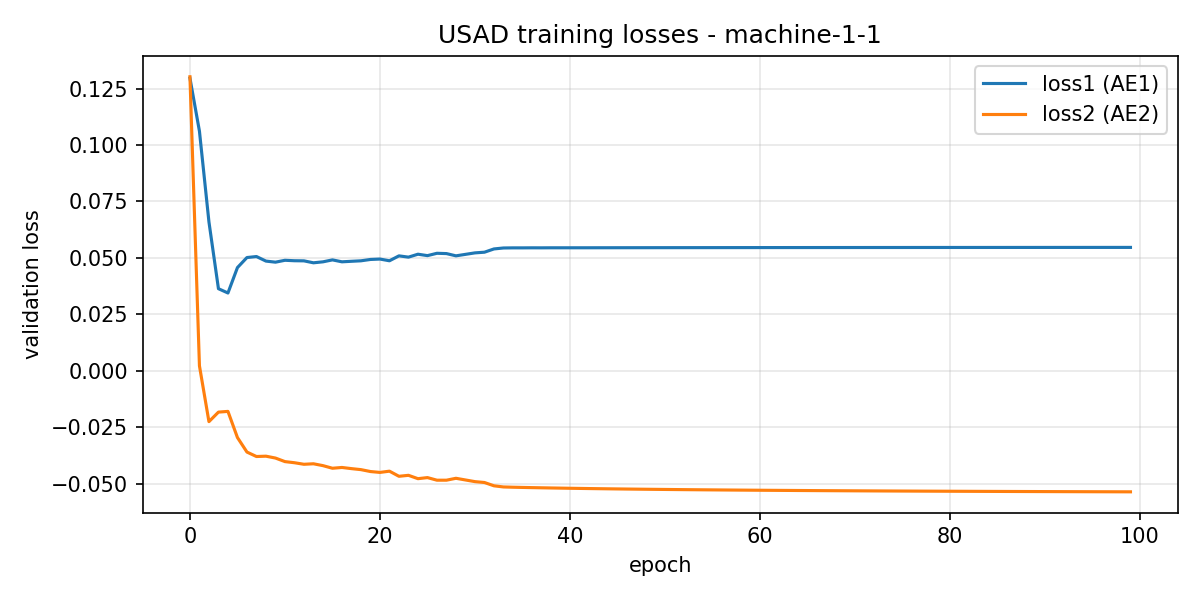
\includegraphics[width=0.92\columnwidth]{figures/fig_losses.png}
\caption{Validation losses of $AE_1$ and $AE_2$ on SMD machine-1-1. Both converge smoothly; $\mathcal{L}_{AE_2}$ goes negative by design.}
\label{fig:losses}
\end{figure}

\begin{table}[t]
\centering\small
\setlength{\tabcolsep}{4pt}
\begin{tabular}{llcccc}
\toprule
 & & $P$ & $R$ & F1 & F1* \\
\midrule
Paper & PA & 0.931 & 0.962 & 0.938 & 0.946 \\
\midrule
\multirow{2}{*}{Mine} & PA & 0.792 & 0.736 & 0.723 & 0.763 \\
 & no PA & 0.591 & 0.476 & 0.461 & 0.528 \\
\bottomrule
\end{tabular}
\caption{USAD on all 28 SMD machines. $P$, $R$, F1 are means over machines; F1* is the F1 of mean $P$ and $R$. Mean ROC AUC is 0.772.}
\label{tab:smd}
\end{table}

\paragraph{Results.} Table~\ref{tab:smd} compares my results with the paper. Replication is \emph{partial}: with PA, I reach F1* = 0.763 against 0.946 in the paper. Figure~\ref{fig:permachine} shows that the mean hides a wide spread:
\begin{itemize}
\item 9 of 28 machines reach F1 $\geq$ 0.9 with PA, and two (2-8 and 3-11) reach 1.0.
\item 7 machines score below 0.5; the lowest is machine 3-3 at 0.27.
\item Without PA, every machine drops, often by half. Machine 1-1 falls from 0.92 to 0.40, and F1* falls to 0.528.
\end{itemize}
Figure~\ref{fig:smdscore} shows why for machine 1-1: the score rises inside most labelled segments but crosses the threshold for only part of each one, which PA then credits as a full detection.

\begin{figure*}[t]
\centering
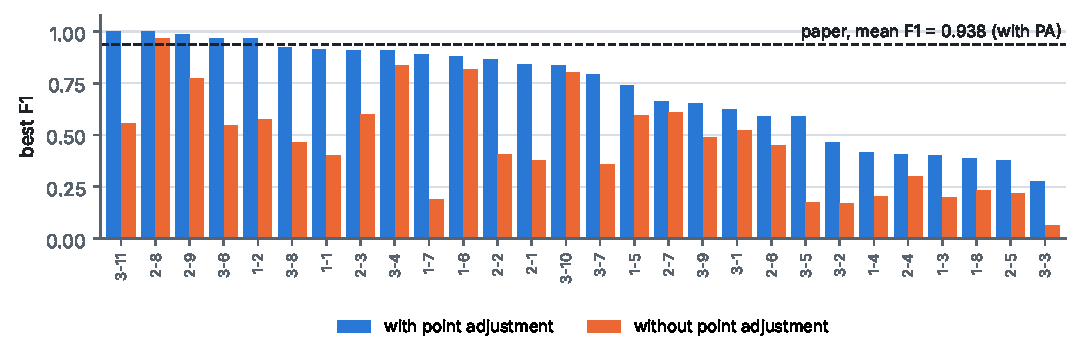
\includegraphics[width=0.95\textwidth]{figures/fig_smd_per_machine.pdf}
\caption{Best F1 per SMD machine, with and without point adjustment, sorted by the PA score. The dashed line is the paper's reported F1.}
\label{fig:permachine}
\end{figure*}

\begin{figure}[t]
\centering
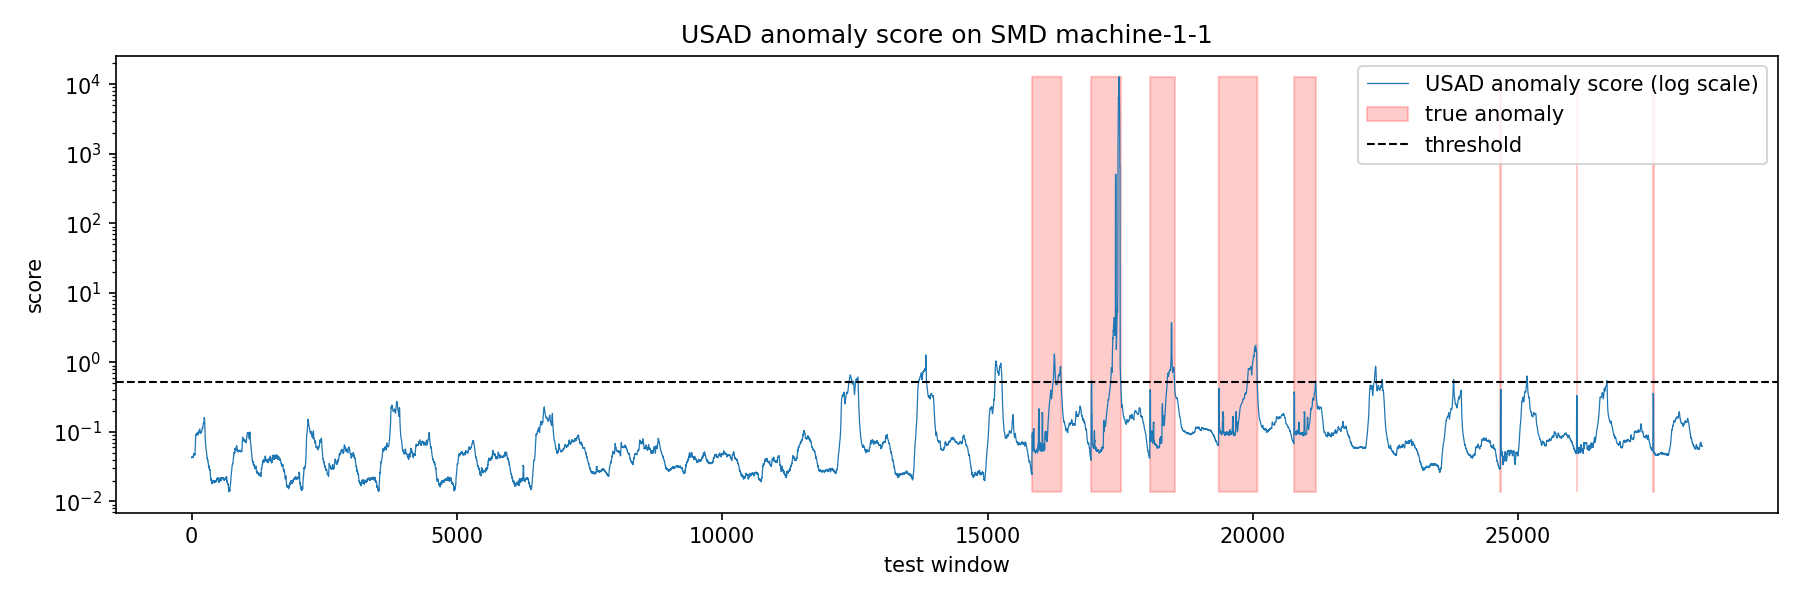
\includegraphics[width=\columnwidth]{figures/fig_smd_scores.png}
\caption{USAD score (log scale) on SMD machine-1-1 test data, with labelled anomalies (red) and the best-F1 PA threshold.}
\label{fig:smdscore}
\end{figure}

\paragraph{Why the results are not closer.} I see five plausible causes, in rough order of importance.
\begin{enumerate}
\item \textbf{Hyperparameters.} The paper tunes the window size and the $\alpha/\beta$ weights per dataset. I used the notebook defaults built for SWaT, and the paper itself reports a sensitivity analysis for these parameters.
\item \textbf{Protocol details the paper does not fully specify.} It does not say how window scores map back to points, which threshold grid it searches, or exactly how F1 and F1* are aggregated. My window-level labelling (any anomalous point marks the window) is one reasonable choice among several.
\item \textbf{Threshold search.} The paper's search over thresholds may be finer than my 300 quantiles, and best-F1 search is sensitive to it.
\item \textbf{One seed.} I trained each machine once, while the large per-machine variance suggests results move between runs.
\item \textbf{Software drift.} The code targets PyTorch 1.6, while I ran a current version.
\end{enumerate}
I found no error in the official code. The authors' later work also questions whether deep models clearly beat simple baselines on these benchmarks \citep{audibert2022deep}, which is consistent with how fragile the headline numbers are.

% =====================================================================
\section{Construction of New Data}
\label{sec:newdata}

\subsection{Existing dataset: SKAB}
SKAB\footnote{\url{https://github.com/waico/SKAB}} \citep{katser2020skab} is an industrial water-circulation testbed recorded once per second with eight sensors (two accelerometers, current, pressure, two temperatures, voltage and flow rate). It contains one anomaly-free run of 9,405 rows and 34 labelled experiments (16 \texttt{valve1}, 4 \texttt{valve2}, 14 \texttt{other}). Together the experiments hold 37,401 rows, 35\% of them anomalous, where faults such as valve closures and pump disturbances were staged.

SKAB is close in spirit to SWaT but needs no access request, so it fits the paper's industrial setting. It was not used in the paper. Each file is \texttt{;}-separated with an \texttt{anomaly} label per row (Figure~\ref{fig:snip-skab}). My preprocessing:
\begin{itemize}
\item I drop the \texttt{changepoint} column.
\item I fit the scaler on the anomaly-free run, train one USAD model on it, and score every experiment file separately.
\item Test values are clipped to $[-5, 5]$ after scaling, because some experiments go far outside the normal range.
\end{itemize}
Exathlon \citep{jacob2021exathlon}, my second proposed candidate, was dropped for time. It needs a much heavier pipeline (93 high-dimensional Spark traces), and SKAB plus the constructed dataset already cover the proposal's two new-data requirements.

\begin{figure}[t]
\centering
\scriptsize
\begin{verbatim}
datetime;Accelerometer1RMS;...;Current;
  Pressure;Temperature;...;
  Volume Flow RateRMS;anomaly;changepoint
2020-03-09 10:14:33;0.0265878;...;1.3302;0.054711;
  79.3366;...;32.0;0.0;0.0
\end{verbatim}
\vspace{-1.5em}
\caption{A row of SKAB \texttt{valve1/0.csv} (abridged).}
\label{fig:snip-skab}
\end{figure}

\subsection{Constructed dataset: household power with injected anomalies}
Real multivariate data with trustworthy anomaly labels is scarce, and labelling it by hand would need domain experts I do not have. I therefore built a dataset whose labels are correct \emph{by construction}: I start from real but unlabelled readings and inject anomalies with known type, timing and severity. The pipeline is a fixed-seed script (seed 42) in the repository.

\paragraph{Collection.} The UCI Individual Household Electric Power Consumption data\footnote{\url{https://doi.org/10.24432/C58K54}} \citep{hebrail2012} has 2,075,259 one-minute readings from one house near Paris (Dec 2006 -- Nov 2010). It has 7 channels: active and reactive power, voltage, current intensity, and three sub-meters for the kitchen, laundry and water heater/air-conditioner. 1.25\% of rows are missing, and there are no anomaly labels. Its domain (smart-home IoT) differs from both SMD and SKAB.

\paragraph{Preprocessing.} I resampled to 10-minute means, which gives 207,527 steps while keeping daily patterns. Gaps of up to one hour were filled by time interpolation. Longer outages were also interpolated but flagged, and kept out of injection. The data was then split by date into a clean training period (2007-01-01 to 2009-06-30, 131,328 steps) and a test period (2009-07-01 onwards, 73,999 steps).

\paragraph{Annotation by injection.} Into the test period I injected 20 segments of each of four types, each type at low or high severity. Segments never overlap, are at least a day apart and avoid imputed outages.
\begin{itemize}
\item \textbf{Spike} (1--3 steps): a channel jumps by 3$\sigma$ (low) or 6$\sigma$ (high).
\item \textbf{Drift} (6--24 hours): a linear offset that ramps up to 2$\sigma$ or 4$\sigma$.
\item \textbf{Dropout} (2--12 hours): one channel (low) or all channels (high) read 0, as in a meter failure.
\item \textbf{Decoupling} (4--12 hours): current is replaced, 50\% (low) or 100\% (high), by its value from a different week. This breaks its physical link to active power while each channel still looks plausible on its own, much like the spoofed sensor in SWaT.
\end{itemize}
These 80 segments cover 4.59\% of test steps, and every one is recorded in an injection log with type, channel, severity, start and end (Figure~\ref{fig:inj}; snippet in Appendix~\ref{app:snips}).

\paragraph{Quality and agreement.} Labels come from the generator, so no human annotation was needed, and agreement with ground truth is exact by definition. I verified the dataset in two ways:
\begin{itemize}
\item Re-running the script outside Colab reproduced the injection log byte for byte.
\item The LLM-as-judge study (Section~\ref{sec:judge}) is an independent check that the injected anomalies are recognisable in the data. Its agreement with the injection log is $\kappa$ = 0.88.
\end{itemize}
Compared with SMD, the constructed data is smaller and has synthetic anomalies, but it offers what SMD's expert labels cannot: per-type and per-severity ground truth.

\begin{figure}[t]
\centering
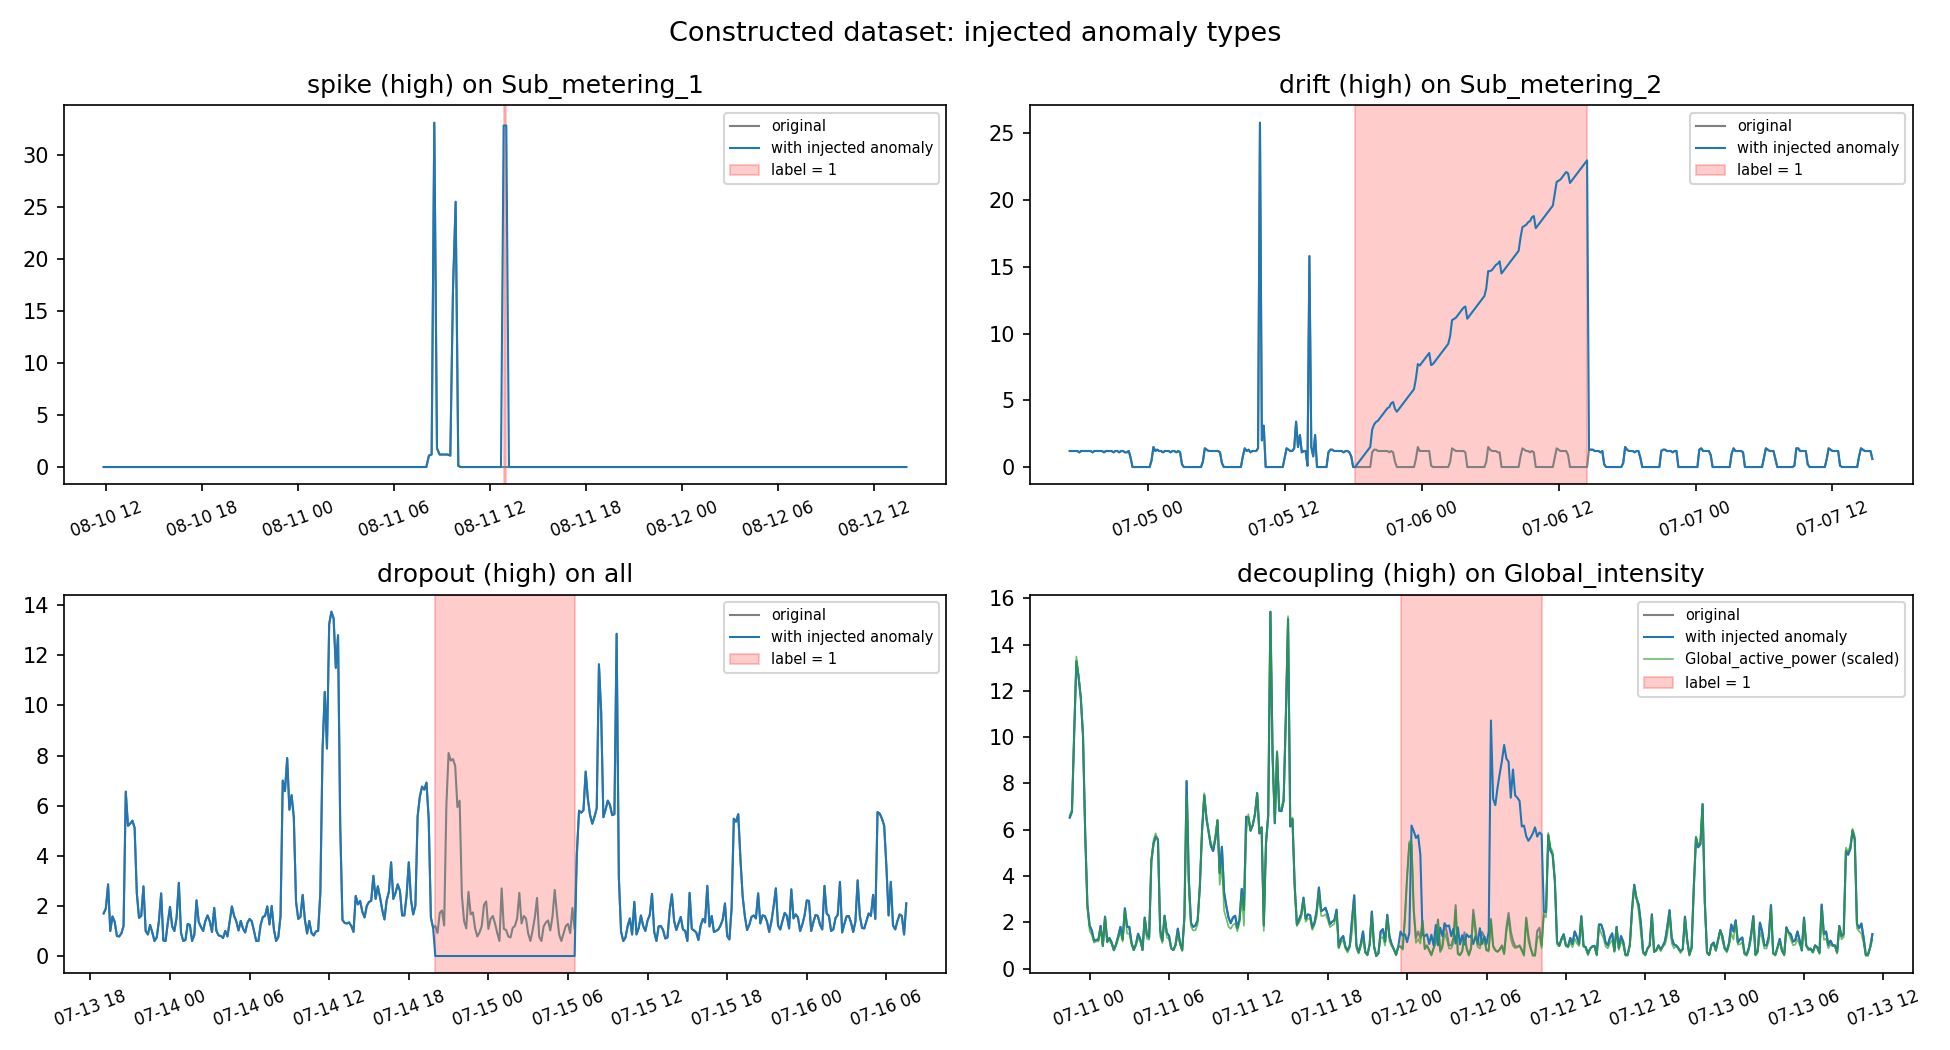
\includegraphics[width=\columnwidth]{figures/fig_injection_examples.png}
\caption{One high-severity example of each injected type: original (grey), after injection (blue), label (red band).}
\label{fig:inj}
\end{figure}

% =====================================================================
\section{Results on New Data}
\label{sec:resnew}

Both new datasets use exactly the replication's settings and evaluation code, so the numbers are directly comparable (Table~\ref{tab:all}). One difference: SKAB is scored per file and averaged, as SMD is per machine, while the UCI data is a single series.

\begin{table}[t]
\centering\small
\setlength{\tabcolsep}{3.2pt}
\begin{tabular}{llcccc}
\toprule
Data & & $P$ & $R$ & F1 / F1* & AUC \\
\midrule
SMD & PA & 0.792 & 0.736 & 0.763* & \multirow{2}{*}{0.772} \\
 & no PA & 0.591 & 0.476 & 0.528* & \\
\midrule
SKAB & PA & 0.947 & 1.000 & 0.973* & \multirow{2}{*}{0.671} \\
 & no PA & 0.602 & 0.929 & 0.730* & \\
\midrule
UCI & PA & 0.538 & 0.433 & 0.480 & \multirow{2}{*}{0.639} \\
 & no PA & 0.497 & 0.188 & 0.273 & \\
\bottomrule
\end{tabular}
\caption{USAD with identical settings on the original and new data. * = F1*; UCI is a single series, so plain F1 is given.}
\label{tab:all}
\end{table}

\paragraph{SKAB.} With PA, SKAB looks almost perfect: F1* is 0.973, and 20 of 34 files score F1 = 1.0. This is mostly an artefact. SKAB's anomalies are long, about a third of each file, so flagging a single point in each segment earns full recall. AUC, which does not depend on a threshold, tells a different story:
\begin{itemize}
\item On the \texttt{other} experiments, mean AUC is 0.865 and USAD ranks anomalies well.
\item On \texttt{valve1} and \texttt{valve2}, mean AUC is 0.528 and 0.561, close to chance (Figure~\ref{fig:skab}).
\end{itemize}
The valve experiments seem to run in a different operating regime from the single anomaly-free run, so most of each file looks unfamiliar to the model, and normal and anomalous windows both score high. This is a distribution-shift failure that the paper's evaluation cannot reveal: on SMD, train and test come from the same machine and regime.

\begin{figure}[t]
\centering
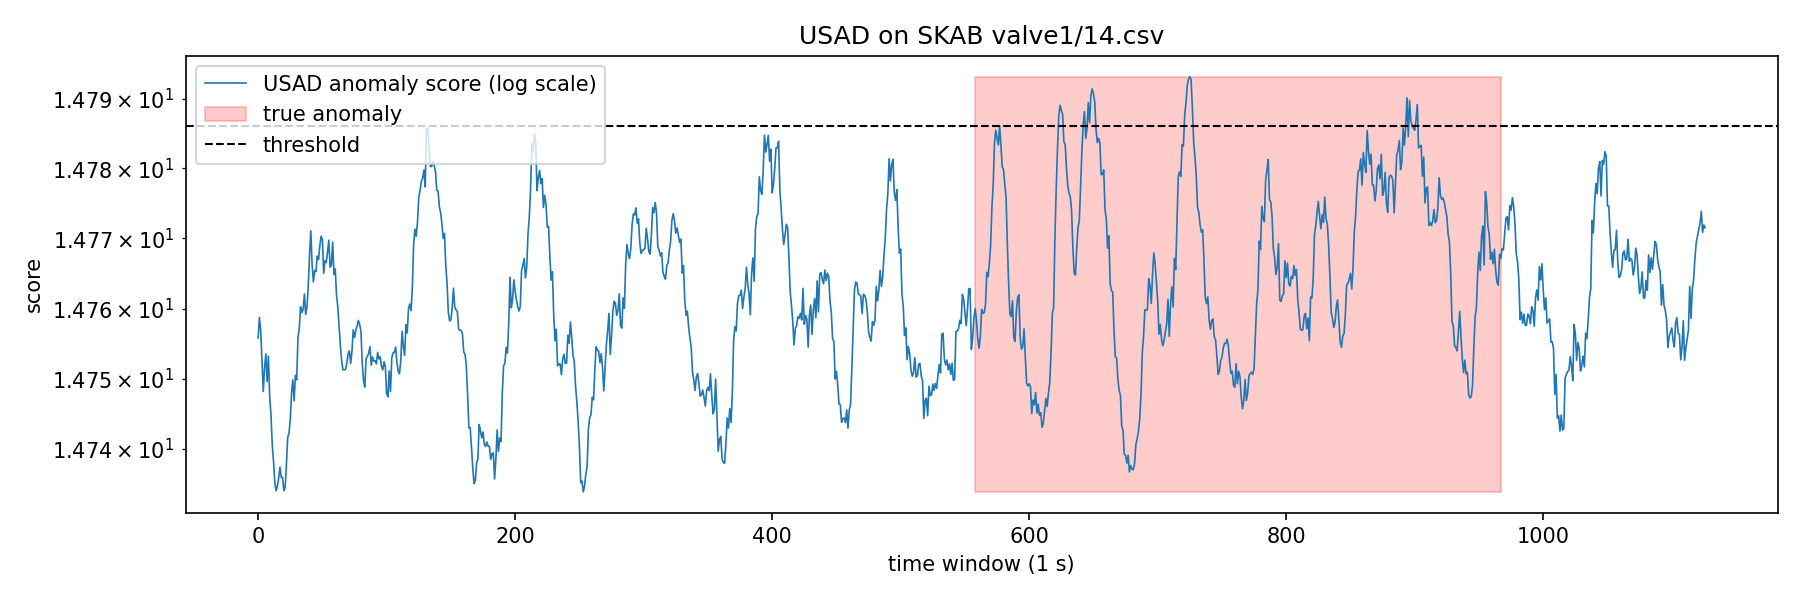
\includegraphics[width=\columnwidth]{figures/fig_skab_scores.png}
\caption{USAD score on a typical SKAB valve experiment: scores are high throughout, so the threshold cannot separate the labelled anomaly.}
\label{fig:skab}
\end{figure}

\paragraph{Constructed UCI dataset.} This is the hardest of the three datasets, with F1 of 0.480 with PA and 0.273 without, and AUC of 0.639. The per-type breakdown (Figure~\ref{fig:typejudge}a, at the best no-PA threshold) explains why; overall, USAD detects 24 of the 80 segments.
\begin{itemize}
\item \textbf{Dropouts:} every high-severity (all-channel) dropout is caught, but none of the single-channel ones.
\item \textbf{Drifts:} 55\% of high-severity and 22\% of low-severity drifts are caught.
\item \textbf{Spikes and decouplings:} almost none are caught (5\% each).
\end{itemize}
The 10-minute averaging and the household's naturally large appliance spikes plausibly hide injected spikes. The decoupling result is the most informative. It is exactly the cross-channel inconsistency that a multivariate detector is meant to catch and that motivated the method in my proposal, yet USAD misses it: its reconstruction error is dominated by each channel's own magnitude, and swapped-in current values stay within a normal range.

Compared with the replication, USAD generalises reasonably to data like its training distribution (the SKAB \texttt{other} files, AUC 0.865) but struggles with regime shift (SKAB valves) and with subtle multivariate anomalies (UCI). PA hides both problems.

\begin{figure*}[t]
\centering
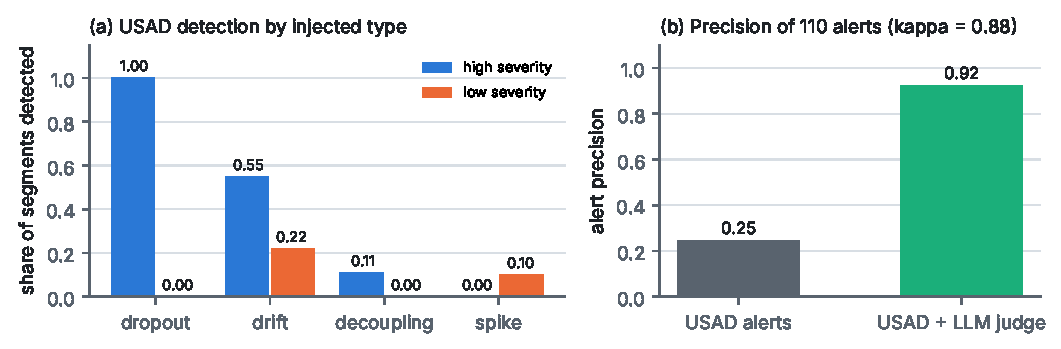
\includegraphics[width=0.88\textwidth]{figures/fig_uci_type_and_judge.pdf}
\caption{(a) Share of injected UCI segments USAD detects, by type and severity. (b) Precision of USAD's 110 alerts on UCI before and after filtering by the LLM judge.}
\label{fig:typejudge}
\end{figure*}

\subsection{LLM-as-judge}
\label{sec:judge}
\paragraph{Design.} I used an LLM to review USAD's alerts. This tests whether an LLM's judgement can stand in for, or add to, human review of detected segments, which is the costly step in real monitoring.
\begin{itemize}
\item At the best no-PA threshold, runs of flagged UCI windows (merged when fewer than 6 windows apart) give \textbf{110 alerts}. Matched against the hidden injection log, 27 are true anomalies and 83 are false alarms.
\item For each alert, a script writes a prompt with the raw values of all seven channels during the alert and two hours either side (downsampled to 20 points), the median value for that hour of day in the training period, and the current/power ratio. It also gives a short, label-free description of the channels and their physics (Appendix~\ref{app:judge}).
\item Prompts carry no dates, labels or injection details, and items are shuffled with random IDs.
\item The judge answers in JSON: \texttt{anomaly}/\texttt{normal}, a type, a 1--5 confidence and a one-sentence rationale.
\item Verdicts were produced by Claude Opus 5.5 and scored against the key only after all 110 were written.
\end{itemize}

\paragraph{Results.} The judge agrees closely with the ground truth: accuracy is 0.955, precision 0.923, recall 0.889, and Cohen's $\kappa$ = 0.88 \citep{cohen1960}. When the judge and the log both call an alert an anomaly, the judge names the right type in 23 of 24 cases. Its confidence is informative: all 21 confidence-5 verdicts were correct, against 14 of 17 at confidence 3. There were five errors:
\begin{itemize}
\item \textbf{Two false positives.} In one, a real current/power break sat just outside the alert window; in the other, the judge mistook a sub-meter's zero standby reading for a dropout.
\item \textbf{Three misses:} two subtle drifts and one low spike.
\end{itemize}
Used as a filter on USAD's alerts, the judge keeps 21 of the 24 true segments and discards 81 of 83 false alarms, raising alert precision from 0.25 to 0.92 (Figure~\ref{fig:typejudge}b).

This complements the ground-truth labels rather than replacing them. The LLM is good at the physical-consistency reasoning that USAD lacks: zero voltage while power is drawn, sub-meters exceeding the total, current not tracking power. But it only sees what USAD flags, so it cannot recover the 56 segments USAD missed.

\paragraph{Caveats.} The verdicts come from one model and one pass, and the same assistant also helped build the pipeline. Prompts were label-free, but full blindness cannot be guaranteed. The repository includes a script that reruns the identical prompts through an API in a fresh context, so the result can be checked with other models or repeated runs. LLM judges have known biases \citep{zheng2023judging}, and a human rater on a subset would be the natural next check.

% =====================================================================
\section{Ethical Considerations}
\label{sec:ethics}

\paragraph{The original paper.} SMD comes from a commercial data centre and is released with anonymised machine IDs and normalised metrics, so it carries little privacy risk. SWaT and WADI are gated because they describe attacks on critical infrastructure; reporting on detection is low-risk, but the attack descriptions are dual-use. The bigger concern is research integrity. Headline results that depend on point adjustment and best-F1 thresholds chosen with test labels overstate real-world performance \citep{kim2022rigorous,wu2023flawed}, and a deployed detector tuned to look good this way could give operators false confidence or flood them with alarms. My replication shows the effect is large: F1* drops from 0.763 to 0.528 when PA is removed.

\paragraph{Publishing on my new data.} Under the Australian Code for the Responsible Conduct of Research \citep{nhmrc2018code}, several principles apply:
\begin{itemize}
\item \textbf{Honesty and rigour (P1, P2).} I must report the unflattering numbers as prominently as the flattering ones, so this report gives every result with and without PA, alongside AUC, and states that replication was only partial.
\item \textbf{Transparency (P3).} Code, seeds, settings, the injection log and every LLM prompt and verdict are public. The use of generative AI, both as the experimental judge and as a writing and coding aid, is declared here and in the repository.
\item \textbf{Respect and data governance (P5).} The UCI data records one real household's electricity use at one-minute resolution, which can reveal when residents are home, asleep or cooking. Although it is anonymous, public and CC BY 4.0, a publication should not attempt re-identification or describe residents' routines beyond what the analysis needs. I do not redistribute the raw file; a script downloads it from the source.
\item \textbf{Recognition and accountability (P6, P7).} I credit and respect the licences of the dataset creators and the USAD authors (MIT for SMD, GPL-3.0 for SKAB, CC BY 4.0 for UCI, BSD-3 for the code).
\end{itemize}

Injected anomalies are synthetic and must be labelled as such, so no one mistakes them for real faults. The LLM judge raises an accountability issue of its own. Its 0.92 precision is attractive, but if it were used to silently suppress alarms in a real system, a missed fault (it missed 3 of 27 true alerts here) would have no human owner. A responsible design keeps a human in the loop and logs the judge's rationale.

% =====================================================================
\section{Conclusions and Reflections}
\label{sec:concl}

\textbf{Replication was partially successful.} The official USAD code runs unmodified on all 28 SMD machines and trains stably and quickly, but it reaches F1* = 0.763 against the paper's 0.946. Without per-dataset tuning and a fully specified protocol, I could not close the gap, and removing point adjustment drops F1* to 0.528.

\textbf{On new data, USAD generalises unevenly.} On SKAB, it ranks anomalies well when test conditions match training but is near chance under regime shift. On the constructed household dataset, it catches gross failures such as all-channel dropouts and large drifts but misses spikes and correlation breaks, the cases a multivariate method should handle best. In both datasets, point adjustment made performance look better than ranking quality supports.

\textbf{An LLM judge reviewed alerts well} ($\kappa$ = 0.88) and could make USAD far more usable as a filter, with alert precision rising from 0.25 to 0.92.

\paragraph{Reflections.}
\begin{itemize}
\item \textbf{Report both settings from the start.} Seeing how far numbers move with point adjustment, I would now report AUC and non-PA F1 from day one rather than treating them as secondary.
\item \textbf{Get more from the constructed data.} Constructing data by injection gave clean, fine-grained labels and was far more informative than I expected. I would add a second household and compare severities on a continuous scale.
\item \textbf{Tune, and run more seeds.} A small hyperparameter search and several seeds per machine would have been the most valuable use of extra time, because they address the largest likely causes of the replication gap.
\item \textbf{Annotation is subtle even with an LLM.} One of the judge's errors was a pattern just outside the alert window. Deciding what counts as ``the alert'' turned out to matter as much as the judge itself.
\end{itemize}

\bibliography{custom}

\appendix
\section{Data Snippets}
\label{app:snips}
{\scriptsize
\begin{verbatim}
Raw UCI file (one-minute readings, ';'-separated):
Date;Time;Global_active_power;
  Global_reactive_power;Voltage;
  Global_intensity;Sub_metering_1;
  Sub_metering_2;Sub_metering_3
16/12/2006;17:24:00;4.216;0.418;
  234.840;18.400;0.000;1.000;17.000

Constructed test set (10-min means + label):
datetime,Global_active_power,...,label
2009-07-01 00:00:00,0.224,0.036,243.585,
  0.96,0.0,0.0,0.6,0

Injection log (ground truth):
id,type,channel,severity,start,end,
  start_idx,end_idx,length_steps
0,drift,Sub_metering_2,high,
  2009-07-05 18:10,2009-07-06 14:30,
  685,808,123
32,decoupling,Global_intensity,high,
  2009-07-11 23:30,2009-07-12 10:10,
  1581,1646,65
\end{verbatim}}

\section{LLM-as-Judge Prompt and Example}
\label{app:judge}
The system prompt (abridged) describes the seven channels, notes that current physically tracks active power ($I/P \approx 4.1$--$4.4$), says that normal household load is bursty but physically consistent, and defines the four anomaly types. It asks for a JSON verdict. An abridged user prompt and answer, for item A078:
{\scriptsize
\begin{verbatim}
Alert length: 23 steps (230 min),
  starting Monday 09:40.
Global_active_power: before mean 4.35 |
  alert mean 5.14 ...
   series: 5.17 4.38 4.17 4.25 4.38 ...
Global_intensity: before mean 6.63 |
  alert mean 7.11 ...
I/P ratio series: 2.12 1.69 1.41 1.42
  1.39 ... 0.57 ...

{"verdict": "anomaly",
 "type": "decoupling", "confidence": 5,
 "rationale": "Current is far too low
  for the active power for hours (I/P
  about 0.6-2.4 instead of about 4.2),
  so current has stopped tracking
  power."}
\end{verbatim}}
\noindent The key confirms this alert as an injected high-severity decoupling. All 110 prompts, verdicts and the scoring script are in the repository.

\end{document}
